\documentclass[12pt]{report}
\usepackage[utf8]{inputenc}
%\usepackage[T1]{fontenc}
\usepackage{tgbonum}
\usepackage[english]{babel}
\usepackage{graphicx}
\usepackage{amsmath}
\usepackage{amssymb}
\usepackage{hyperref}
\usepackage{epsf}
\usepackage{float}
\usepackage{mathpazo}
\usepackage{pifont}
\usepackage{color}
\definecolor{mygreen}{RGB}{70, 180, 90}
\definecolor{mylilas}{RGB}{255, 117, 45}
\definecolor{cadr}{rgb}{0.89, 0.0, 0.13}
\definecolor{myblue}{RGB}{0, 102, 204}
\usepackage{caption}
\usepackage{subcaption}
\usepackage{subfloat}
\usepackage
[
a4paper,% other options: a3paper, a5paper, etc
left=3cm,
right=3cm,
top=3cm,
bottom=3cm,
]{geometry}
%\geometry{hmargin=3.5cm, vmargin=2.5cm}
\usepackage{fancyhdr}
\pagestyle{fancy}
\fancyhf{}
\rfoot{\thepage}
\renewcommand{\headrulewidth}{0pt}
\usepackage{color}
\graphicspath{{figures/}}
\usepackage{graphicx}
\usepackage{wrapfig}
\usepackage{graphicx}
\usepackage{multicol}
\usepackage{enumitem}
\usepackage{xcolor}
\usepackage{framed}
\usepackage{bm}
\definecolor{shadecolor}{RGB}{139, 231, 3}
\usepackage{epigraph}

\usepackage{mathpazo}
\usepackage[framemethod=TikZ]{mdframed}
\usepackage{lipsum}

\usepackage{color}
\definecolor{color-box-border-equation}{RGB}{200,200,200}
\definecolor{color-box-background-equation}{RGB}{250,250,250}

\definecolor{color-box-border-code}{RGB}{54,119,168}
\definecolor{color-box-background-code}{RGB}{236,245,255}

\mdfdefinestyle{equation-frame}{%
    linecolor=color-box-border-equation,
    outerlinewidth=1pt,
    roundcorner=10pt,
    innertopmargin=\baselineskip,
    innerbottommargin=\baselineskip,
    innerrightmargin=20pt,
    innerleftmargin=20pt,
    backgroundcolor=color-box-background-equation}
    
\mdfdefinestyle{exercise-frame}{%
    linecolor=color-box-border-code,
    outerlinewidth=1pt,
    roundcorner=10pt,
    innertopmargin=\baselineskip,
    innerbottommargin=\baselineskip,
    innerrightmargin=20pt,
    innerleftmargin=20pt,
    backgroundcolor=color-box-background-code}

\usepackage{pifont}

\usepackage{tcolorbox}
\definecolor{mycolor}{rgb}{0.122, 0.435, 0.698}

\newtcbox{\mb}{nobeforeafter,colframe=mycolor,colback=mycolor!10!white,boxrule=0.5pt,arc=4pt,
  boxsep=0pt,left=6pt,right=6pt,top=3pt,bottom=3pt,tcbox raise base}

\usepackage{eso-pic}
\newcommand\BackgroundPic{%
\put(-50,-0){%
\parbox[b][\paperheight]{\paperwidth}{%
\vfill
\centering
\includegraphics[height=\paperheight,%
keepaspectratio]{figures/cover.png}%
\vfill
}}}

%\usepackage{emerald}
\usepackage[T1]{fontenc}

\usepackage{anyfontsize}
\usepackage{t1enc}
\newcommand{\heart}{\ensuremath\varheartsuit}
\usepackage{tikz}
\usetikzlibrary{positioning}

% CHAPTER STYLE =================================================

\makeatletter
\def\thickhrulefill{\leavevmode \leaders \hrule height 1ex \hfill \kern \z@}
\def\@makechapterhead#1{%
  \vspace*{10\p@}%
  {\parindent \z@ \raggedleft \reset@font
            \scshape \@chapapp{} \thechapter
        \par\nobreak
        \interlinepenalty\@M
    \Huge \bfseries #1\par\nobreak
    %\vspace*{1\p@}%
    %\hrulefill
    \par\nobreak
    \vskip 50\p@
  }}
\def\@makeschapterhead#1{%
  \vspace*{10\p@}%
  {\parindent \z@ \raggedleft \reset@font
            \scshape \vphantom{\@chapapp{} \thechapter}
        \par\nobreak
        \interlinepenalty\@M
    \Huge \bfseries #1\par\nobreak
    %\vspace*{1\p@}%
    %\hrulefill
    \par\nobreak
    \vskip 50\p@
  }}

\begin{document}

% TITLE PAGE ====================================================

\begin{titlepage}
\AddToShipoutPicture*{\BackgroundPic}
\ \\[4cm]
{\sffamily \color{white}
\begin{center}
\fontsize{76}{10}\selectfont \fontfamily{qcr}\selectfont Fluid

\vskip 5\p@

\fontsize{55}{10}\selectfont \fontfamily{qcr}\selectfont Toolbox

\vskip 10\p@

%\fontsize{25}{10} \selectfont \fontfamily{augie}\selectfont with Python

\end{center}
}
\vfill
{\fontsize{20}{20}\color{white}\sffamily Kamila Zdybał \hfill\color{white} Zürich, 2025}

{\fontsize{10}{10}\color{white}\sffamily \href{https://kamilazdybal.github.io/}{\texttt{kamilazdybal.github.io}}}
\end{titlepage}


% EX LIBRIS PAGE ================================================

\thispagestyle{empty}
\begin{center}
\vspace*{1cm}
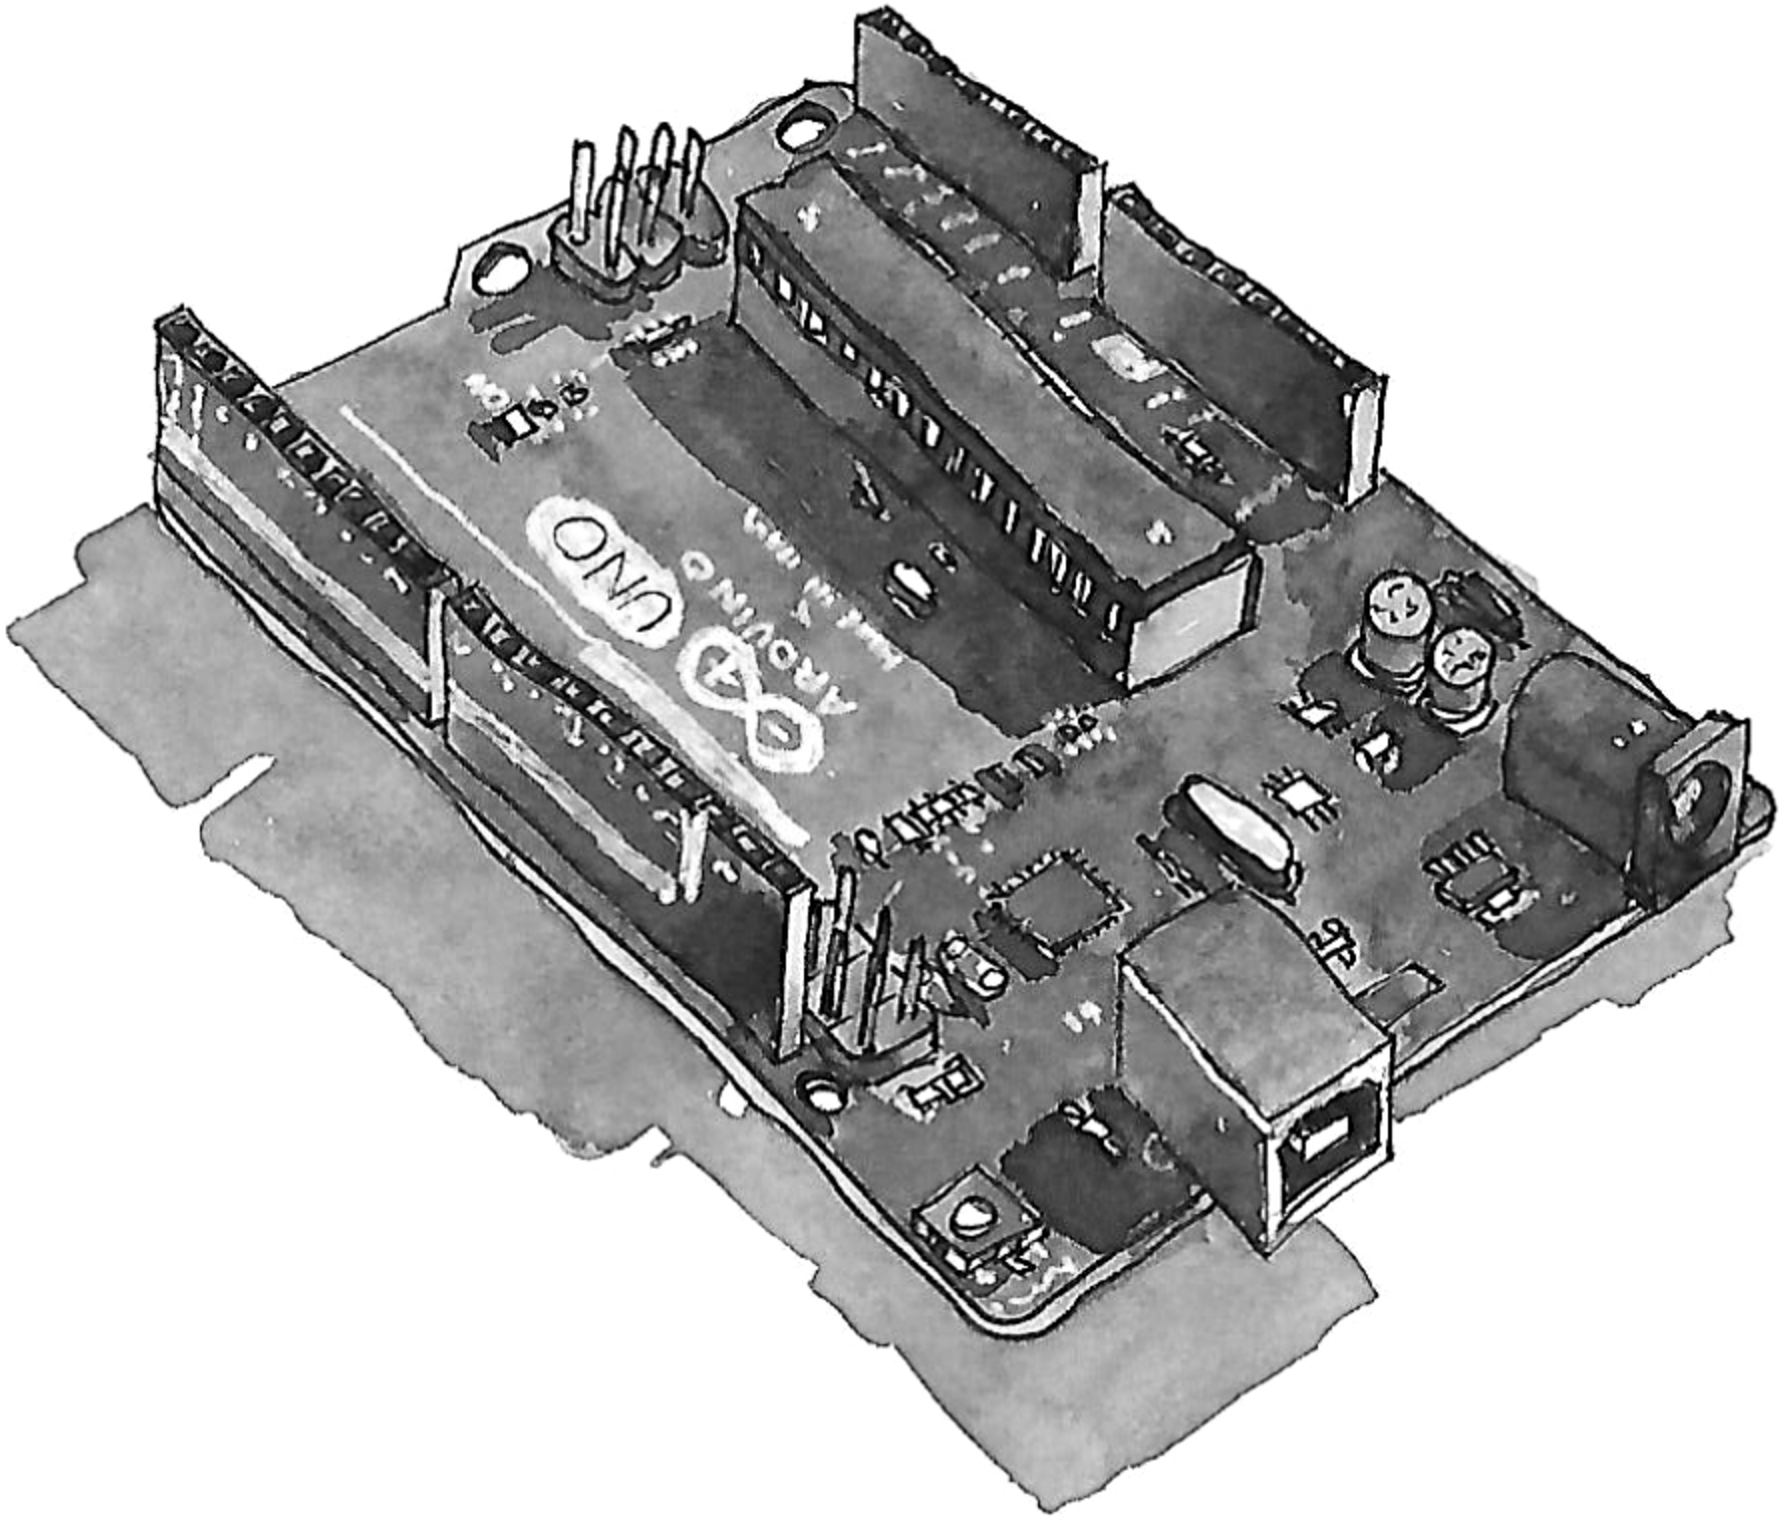
\includegraphics[width = 80mm]{ex_libris_arduino.jpg}

\vspace*{1cm}

{\fontsize{18}{10}\selectfont \fontfamily{pbk}\selectfont E X \,\, L I B R I S $\cdotp$ K A M I L A}

\vspace*{2cm}

Copyright \textcopyright \, K. Zdybał, 2025

For more projects similar to this one

visit my personal website: \verb|kamilazdybal.github.io|

or visit me on GitHub: \verb|@kamilazdybal|

You can contact me with any thoughts, suggestions, or corrections:

\verb|kamilazdybal at gmail dot com|

\vspace*{0.6cm}

This document will be alive for quite some time. 

I will be coming back to it to add or improve things. 

You can always access the newest version through my website.

\vspace*{1.8cm}

\verb|Fluid Toolbox|

\verb|version 1.1|

Typeset with \ding{170} for \LaTeX

\vspace*{1.8cm}

\noindent This work is licensed under the Creative Commons

Attribution-NonCommercial-ShareAlike 4.0 International 

(CC BY-NC-SA
4.0) license.
\end{center}

\setlength{\parskip}{0.6em}
\setlength{\parindent}{0cm}

\chapter*{Preface}
\thispagestyle{empty}
\chaptermark{Preface}

\rightline{{\rm \textit{``Use it well.''}}}

\rightline{{\rm --- Prof. Albus Dumbledore}}

\texttt{\textbf{Fluid Toolbox}} is a collection of human-readable, pseudo-random study notes that inspire you to think deeper about various fluid dynamics concepts. It is meant to be used complimentary to the regular textbook since it may provide additional insights, but it will not substitute the thoroughness of a standard course in the subject. I believe that working side-by-side with a course it can become a useful toolbox of concepts that are ready-to-understand and ready-to-use.

\textbf{Why is this text created?}

I had a goal of collecting in one place the most important fluid dynamics concepts, as well as some prerequisites to studying fluid dynamics. Much of the knowledge presented here comes from my search for understanding that I was often missing when reading textbooks, and which was difficult to find in a way that would be engaging, illustrative, and would make intuitive sense to me. Some of the understanding presented here comes from my personal explorations and thinking on the subject, some of it comes from sources that I found very helpful -- I will make references to those as we go. I have hopes that this document will become a helpful resource that you have been looking for. Above all, I will know that it was worth writing it if you enjoy the journey of reading and learning from it!

\textbf{Some of my thoughts on learning}

I believe in the quote by Richard Feynman: \textit{Study hard what interests you the most in the most undisciplined, irreverent, and original manner possible.} I will sometimes ask a brain-teasing question or challenge you to \textit{pause and ponder}. In your own learning, do challenge yourself, and don't let your imagination be limited by simply following pages of any textbook! When learning a new subject, it's simply not enough to read a textbook or watch a lecture; those are both easy tasks to do. When you become a spectator in the studying process, it's easy to fool yourself that you understood something. The real learning and understanding comes when it's only you, your head, and a blank piece of paper. It is only when you have a chance to take action in your recall of information that you can really use your knowledge and test your deep understanding. Oh, and by the way... Programming is a great way to roll your sleeves and put things into action. So is teaching others!\footnote{And so my sneaky goal is to learn some fluid dynamics writing this document!}

\newpage
\thispagestyle{empty}
\tableofcontents

\newpage
\chapter*{Acknowledgements}
\thispagestyle{empty}
\chaptermark{Ack}

{\fontsize{12}{12}\rightline{\textit{I am grateful to all people I encountered in my life}}}

\vspace*{0.5cm}

{\fontsize{12}{12}\rightline{\textit{who supported my passion for studying fluid motion.}}}

\vspace*{0.5cm}

{\fontsize{12}{12}\rightline{\textit{Among the first ones were Y. Çengel and J. Cimbala}}}

\vspace*{0.5cm}

{\fontsize{12}{12}\rightline{\textit{in their inspiring fluid mechanics textbook.}}}

\vspace*{2cm}
\rightline{{\rm \textit{Zürich, Switzerland, 2025}}}


\newpage

% - - - - - - - - - - - - - - - - - - - - - - - - - - - - - - - - - - - - - - - - - - - - - - - - 
\chapter{Changes} \label{chap:changes}

\rightline{{\rm \textit{Ch-ch-ch-ch-changes}}}
\rightline{{\rm \textit{Turn and face the strange}}}
\rightline{{\rm \textit{Ch-ch-changes}}}
\rightline{{\rm \textit{There's gonna have to be a different man}}}

\rightline{{\rm --- David Bowie}}

In studying fluid motion, we are inherently interested in \textbf{change} in various quantities associated with the fluid. For example, simply because of fluid moving around, its local density or its local temperature might change. With that perspective, the main goal of the science of fluid dynamics is to describe and then calculate that change. Much of the time, we would like to know how flow affects various fluid properties such as its density, pressure, temperature, or even things like mixture composition in multicomponent fluids.
In this Chapter, I discuss the most fundamental building block for talking about change -- \textbf{a derivative}. I hope to show you just how expressive derivatives are in terms of the various types of processes that they can describe!

\section{Derivatives model change}

\textbf{Change} is mathematically modeled by \textbf{derivatives}. A derivative explains how much one variable, say $\varphi$, changes when we change some other variable, say $\psi$, and we express this in mathematical terms as
\begin{equation*}\label{eq:change-d}
\frac{d \varphi}{d \psi} \, ,
\end{equation*}
where the letter $d$ stands for \textit{the change of...} and is later followed by the variable that we are speaking of. So really the above ratio means that there is \textit{this much} change in variable $\varphi$ per \textit{this much} change in variable $\psi$. You can also think of this ratio as \textit{this much} change in variable $\varphi$ per \textit{unit} change in variable $\psi$.

In fluid dynamics, you will find that we are most interested in two types of change: \textit{change in time} and \textit{change in space}. Since we live in a 3D space, with Cartesian coordinates $x$, $y$, and $z$, with a time arrow ($t$), it is justifiable why these two have the biggest popularity, right? Therefore, you will most often encounter $dt$, or $dx$, $dy$, and $dz$, in the denominator of various forms of derivatives.

Let's take pressure, $p$, as an example. When we write
\begin{equation*}\label{eq:change-p}
\frac{d p}{d t} \, ,
\end{equation*}
you can read this as: there is this much change in $p$ per this much change in $t$. Here, we have implicitly assumed that $p = p(t)$, that is, that pressure is only a function of time (and not space).
Similarly, you may encounter expressions like
\begin{equation*}\label{eq:change-p}
\frac{d p}{d x} \,  , \,\, \frac{d p}{d y} \, , \,\, \text{and} \,\, \frac{d p}{d z} \, ,
\end{equation*}
which you can read as: change in $p$ per change in $x$, or $y$, or $z$. 
Here, the assumption was that $p = p(x)$, or $p = p(y)$, or $p = p(z)$, respectively.

The above are what we call \textit{ordinary derivatives}. They assume that the variable can change with respect to only one independent variable. But this does not always need to be the case. 

There is also another mathematical expression for a derivative and it is
\begin{equation*}\label{eq:change-partial}
\frac{\partial \varphi}{\partial \psi} \, .
\end{equation*}
The operator $\partial$ (called ''partial`` or ''del``) also stands for \textit{the change of...} but it also gives you a hint that the variable $\varphi$ can change with the change of variables other than $\psi$. Perhaps it can also change with some $\zeta$ and $\chi$, even though in this particular ratio from above we are only interested in the change with respect to $\psi$.

These are called \textit{partial derivatives}. If a variable is a function of more than one independent variable, say $p = p(x,t)$, we are no longer allowed to use ordinary derivatives to be mathematically precise\footnote{Although we all allow ourselves to be mathematically sloppy sometimes! And that's alright, as long as we remember how to be precise if needed.}. Therefore, if $p = p(x,t)$, and we want to express the change of $p$ with respect to time, we have to write
\begin{equation*}\label{eq:change-partial}
\frac{\partial p}{\partial t}
\end{equation*}
and we can no longer write
\begin{equation*}\label{eq:change-partial}
\frac{d p}{d t} \, .
\end{equation*}


There are what we call \textit{higher-order derivatives}, which can look like this:
\begin{equation*}\label{eq:change-partial-2nd}
\frac{\partial^2 \varphi}{\partial \psi^2} \, .
\end{equation*}
What is their meaning? Well, we can also re-write the above as
\begin{equation*}\label{eq:change-partial}
\frac{\partial}{\partial \psi} \frac{\partial \varphi}{\partial \psi} \, ,
\end{equation*}
and this way it's easier to see that this must have the interpretation of measuring how much the very change in $\varphi$ is changing! In other words, we are describing how the quantity 
\begin{equation*}\label{eq:second-derivative}
\frac{\partial \varphi}{\partial \psi}
\end{equation*}
changes with the change to $\psi$. 

\section{Mixing derivatives signals various transport processes} \label{sec:changes:mixing-derivatives}

The really exciting part begins when we equate derivatives with respect to one quantity to derivatives with respect to other quantity. For instance, we can write that
\begin{equation}\label{eq:dt-propto-dx}
\frac{\partial p}{\partial t} \propto \frac{\partial p}{\partial x}
\end{equation}
for a particular point in space and time, and where the pressure, $p = p(x, t)$.

At first glance, it seems rather bizarre to say that a variable's change in time is proportional to its change in space. In the end, I can imagine a function that varies in space and varies in time, but those variations are completely independent of each other. So what does creating a link between space and time mean...? Let's think about this a little more!

First, we have to come to an agreement where exactly are we measuring $\partial p / \partial t$. With the continuum assumption of fluid dynamics, this is always some point in space, say $Q$. Now that we have selected $Q$, let's look at its local neighborhood to determine how does $p$ vary spatially there. This is what the term $\partial p / \partial x$ describes: How much change in $p$ is there along the spatial $x$-direction? But just the sheer existence of that change does not yet mean that our point $Q$ is going to experience any of it as time goes by! That change simply \textit{is}. If we now wanted it to affect our point $Q$, we need to somehow transport that change over to the location $Q$. And fluid's velocity is a great conveyor of that change! In this case, we have just one spatial dimension, therefore the fluid velocity vector $\vec{\bm{V}} = \langle u \rangle$. If we assume that the velocity component in the $x$-direction, $u$, is the constant of proportionality in Eq.~(\ref{eq:dt-propto-dx}), then we have just described an advection of $p$, which in its full form reads
\begin{equation}\label{eq:advection-of-p}
\frac{\partial p}{\partial t} = - u \frac{\partial p}{\partial x} \, .
\end{equation}
Equating the term $- u \partial p / \partial x$ to the temporal derivative, $\partial p / \partial t$, tells us how much of the spatial change in $p$ is being ``slided over'' to the fixed point in space, $Q$. And the strength of that ``sliding over'' is measured by the velocity component, $u$.

Turns out, the link between time and space, embedded in Eq.~(\ref{eq:advection-of-p}), is necessary when we assume fluid's \textit{movement}. 
As we have seen, a moving fluid can alter a point in time by bringing some spatial change over to that point. Only in the absence of movement can time and space be decoupled and completely independent of one another. It is appreciable that with a relatively simple mathematical description in Eq.~(\ref{eq:advection-of-p}), we have been able to describe this very useful transport phenomena!

A second-order derivative,
\begin{equation*}\label{eq:change-partial-2nd}
\frac{\partial p}{\partial t} = \frac{\partial^2 p}{\partial x^2} \, ,
\end{equation*}
is a model for the \textit{diffusion} of $p$. It describes how much change in $\frac{\partial p}{\partial x}$ are we going to experience along the $x$-direction. While the first-order derivative had the interpretation of how much $p$ is being pushed to the adjacent locations on the $x$-axis, with the second-order derivative we describe what is the strength of that ``pushing'' process.



%\section{What does it mean for a quantity to change in time and in space?}


%\subsection{Steady-state case and a time derivative}

\section{Convention for the sign of a derivative}

For the purpose of this demonstration we will look at the derivative $\frac{dp}{dx}$ -- change in pressure per change in the $x$-axis position -- which is often encountered in fluid dynamics. We will lay the ground for what does it mean for this derivative to be positive, negative or zero, and why the reasoning makes sense.

Suppose that the initial point is marked with \textcolor{myblue}{$(i)$} and it is always a point at coordinate $x$. The point to which we move after one space-step, the final point, is marked with \textcolor{myblue}{$(f)$} and is either at $x+dx$ or $x - dx$ coordinate, depending on the positive or negative change that we decide to make. The direction of the change on the $x$-axis is marked with a blue arrow.

\begin{figure}[H]
\begin{subfigure}[t]{.46\textwidth}
\centering
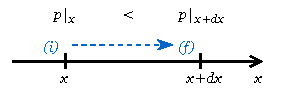
\includegraphics[scale=1]{dp-dx-pos-neg.pdf}
\caption{$\frac{dp}{dx} > 0$ with positive change in $x$.}
\end{subfigure}
\begin{minipage}[t]{.07\textwidth}
$ $
\vspace*{1.5cm}
\end{minipage}
\begin{subfigure}[t]{.46\textwidth}
\centering
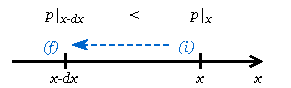
\includegraphics[scale=1]{dp-dx-neg-neg.pdf}
\caption{$\frac{dp}{dx} > 0$ with negative change in $x$.}
\end{subfigure}
\begin{subfigure}[t]{.46\textwidth}
\centering
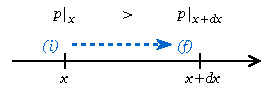
\includegraphics[scale=1]{dp-dx-pos-pos.pdf}
\caption{$\frac{dp}{dx} < 0$ with positive change in $x$.}
\end{subfigure}
\begin{minipage}[t]{.08\textwidth}
$ $
\end{minipage}
\begin{subfigure}[t]{.46\textwidth}
\centering
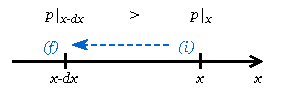
\includegraphics[scale=1]{dp-dx-neg-pos.pdf}
\caption{$\frac{dp}{dx} < 0$ with negative change in $x$.}
\end{subfigure}
\caption{Sign of the $\frac{dp}{dx}$ derivative versus directions of change along the $x$-axis.}
\label{fig:dp-dx-signs}
\end{figure}

We will now find out for all cases which pressure, at \textcolor{myblue}{$(i)$} or at \textcolor{myblue}{$(f)$} must be larger. Our aim is to show that situations (a) and (b) in Figure \ref{fig:dp-dx-signs} must be equivalent -- they explain the same physical phenomena. In both of these cases we will show that the pressure is increasing with the increasing $x$-coordinate, independent of whether we decide to take a step to the right or to the left of our initial point \textcolor{myblue}{$(i)$}. 

We will show the analogical result can be said about situations (c) and (d) but in this case the pressure is decreasing with the increasing $x$-coordinate.

The analysis done in this section is often necessary in order to find out whether or not to ''put a minus sign`` in front of expressions. For instance, as we will show later in the text, such reasoning can help us understand why there is a minus sign in the Euler equation for a fluid element experiencing pressure force: $dp = - \rho \upsilon d \upsilon$. Oftentimes, the sign of a derivative tells an important information about the nature of the physical phenomena.



% - - - - - - - - - - - - - - - - - - - - - - - - - - - - - - - - - - - - - - - - - - - - - - - - 
%\chapter{Differentiation}

%Differentiation is a way to make discrete things continuous.

% - - - - - - - - - - - - - - - - - - - - - - - - - - - - - - - - - - - - - - - - - - - - - - - - 
\chapter{Material derivative}

\section{Where space, time, and fluid flow meet}

The material derivative describes the \textit{total experienced} change in quantity $\bullet$ as \textit{time goes on} \textbf{and} as we \textit{move} across the field of $\bullet$ with fluid velocity, $\vec{\bm{V}} = \langle u, \upsilon, w \rangle$. Hence, the material derivative requires two ingredients; these are visualized in Fig.~\ref{fig:material-derivative-two-ingredients}. The first ingredient is the field of $\bullet$, which can change spatially and temporally (Fig.~\ref{fig:material-derivative-two-ingredients}a). The second ingredient is the associated fluid velocity field, $\vec{\bm{V}}$ (Fig.~\ref{fig:material-derivative-two-ingredients}b). In this chapter, you can substitute for $\bullet$ any interesting physical quantity that you'd like, such as density, $\rho$, or temperature, $T$. Interestingly, this quantity does not need to be a scalar, but can also be a vector or even a tensor.
\begin{figure}[H]
\centering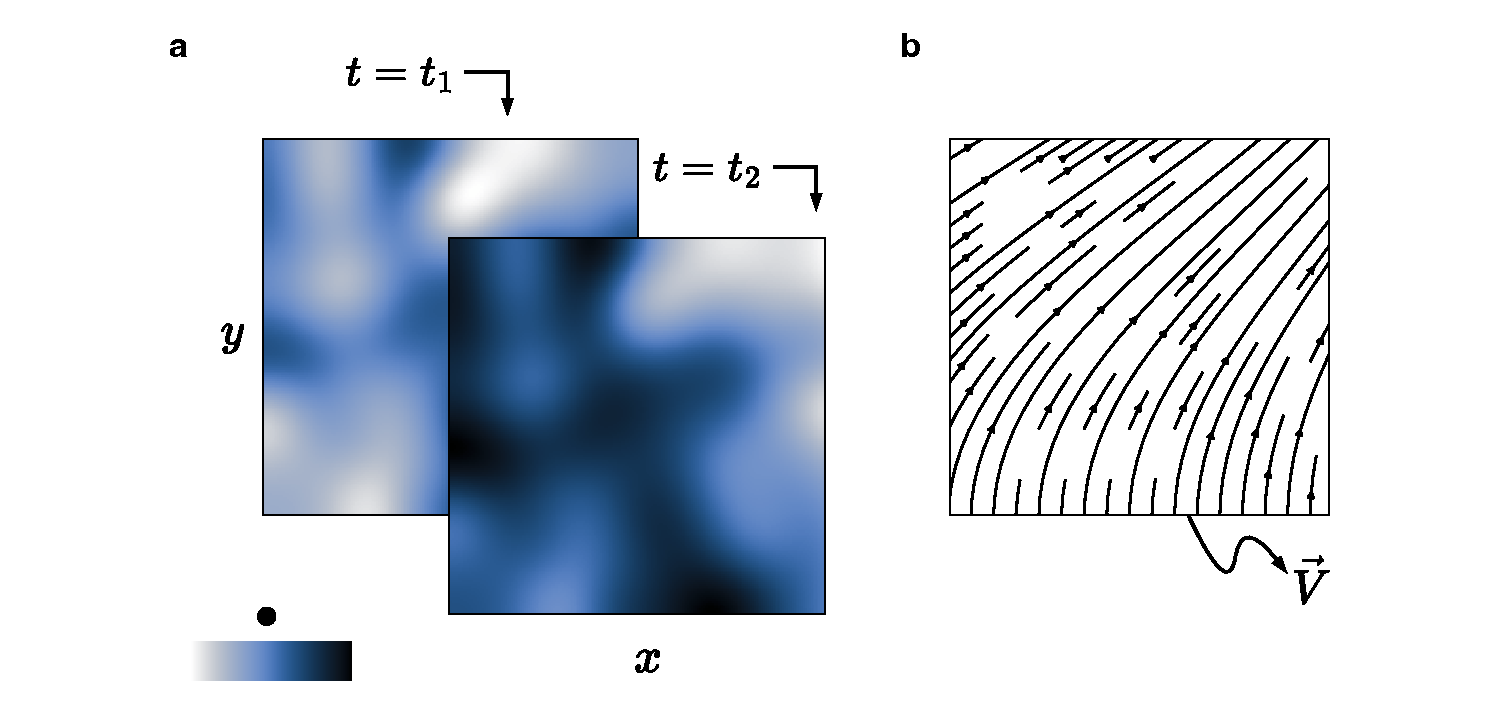
\includegraphics[width=15cm]{material-derivative-two-ingredients.pdf}
\caption{Two ingredients needed to compute the material derivative: (\textbf{a}) the field of $\bullet$, which can change spatially and temporally, and (\textbf{b}) the associated fluid velocity field, $\vec{\bm{V}}$.}
\label{fig:material-derivative-two-ingredients}
\end{figure}

I will start with building a visual intuition for the material derivative. You may consider a 2D field of $\bullet$ that changes in time and space, just like the one presented in Fig.~\ref{fig:material-derivative-two-ingredients}a. In Fig.~\ref{fig:material-derivative-example}, let's look at the possible reasons for why we might experience change in $\bullet$. In the absence of spatial movement over the $(x,y)$ grid we can only experience change in $\bullet$ if $\bullet$ varies in time. Similarly, in the absence of temporal variation in $\bullet$, we can experience change in $\bullet$ only if we travel along the $(x,y)$ grid and $\bullet$ varies over that grid. With both time and motion present, we experience a superposition of these two effects. That will be our total experienced change in $\bullet$.
\begin{figure}[H]
\centering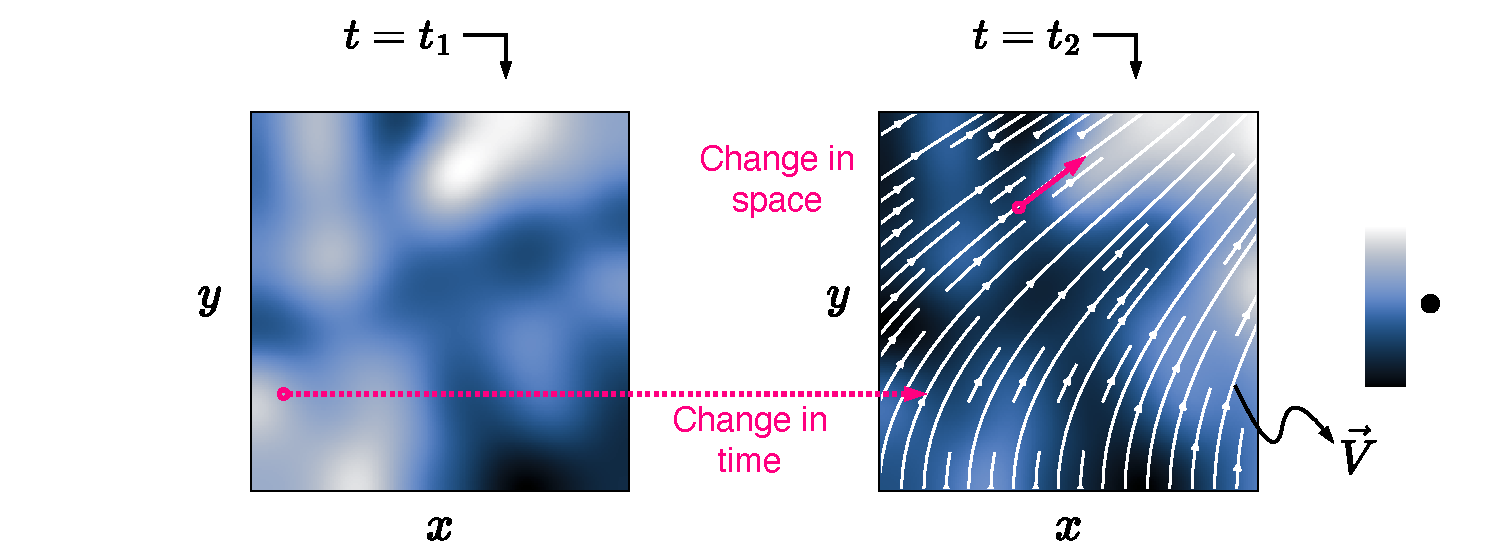
\includegraphics[width=15cm]{material-derivative.pdf}
\caption{A 2D field of some scalar quantity, $\bullet$, that changes in time, $t$, and space, $(x, y)$. We also consider the associated fluid velocity field, $\vec{\bm{V}}$. The material derivative is a superposition of two reasons for why $\bullet$ can change.}			
\label{fig:material-derivative-example}
\end{figure}

In mathematical terms, the material derivative, $\frac{D}{Dt}$, is an operator acting on $\bullet$ such that
\begin{equation} \label{eq:material-derivative}
\frac{D \bullet}{D t} \equiv \frac{\partial \bullet}{\partial t} + \vec{\bm{V}} \cdot \nabla \bullet \, .
\end{equation}
The superposition that I mentioned before is embedded in the two terms on the right-hand-side of Eq.~(\ref{eq:material-derivative}). We can now dissect these two terms to better understand why introducing the material derivative is very useful when studying fluid motion.

First, we have $\frac{\partial \bullet}{\partial t}$ which is the plain old\footnote{See Chapter~\ref{chap:changes}.} partial derivative of $\bullet$ with respect to time. It says that at all possible locations in space, and at any one location, the quantity $\bullet$ can evolve in time. One example of such quantity is temperature. Even if we remain stationary in a specific location, say in a corner of a room, we can still experience change in temperature because our room might be heated (or cooled) and the temperature in our little corner changes in time because of that. The term $\frac{\partial \bullet}{\partial t}$ gives us a recipe for \textit{how} that temperature changes in time in every location of the room.

Second, we have $\vec{\bm{V}} \cdot \nabla \bullet$, that is, a gradient vector, $\nabla \bullet = \langle \frac{\partial \bullet}{\partial x}, \frac{\partial \bullet}{\partial y}, \frac{\partial \bullet}{\partial z} \rangle$, dotted with the fluid velocity vector, $\vec{\bm{V}}$. 
%At this point, you might remind yourself of the intuition behind taking a dot product between two vectors from Fig.~\ref{fig:circulation-dot-product}. 
The gradient of $\bullet$ is a vector field that describes directions in which $\bullet$ varies. If, and only if, our own spatial movement is aligned (at least to some extent) with the direction of $\bullet$'s gradient, we will experience a change in quantity $\bullet$. Otherwise, if we walk along an isocurve of $\bullet$, we will not experience any change in $\bullet$. The dot product taken between $\vec{\bm{V}}$ and $\nabla \bullet$ measures the degree of that alignment.

To summarize, the first term on the right-hand-side of Eq.~(\ref{eq:material-derivative}) describes how we will experience change in $\bullet$ in the absence of our motion through the field of $\bullet$. The second term describes how we will experience additional change in $\bullet$ due to moving around through the field of $\bullet$ but with a very specific velocity, $\vec{\bm{V}}$. I will emphasize again that in the definition of the material derivative our movement is restricted to one defined by the fluid flow. Hence, we specifically use the flow velocity, $\vec{\bm{V}}$, and not any other velocity\footnote{That said, one could, potentially, define a generalization of the material derivative to allow for an arbitrary velocity! Such a new quantity will have a different physical meaning though.}. The material derivative is a neat superposition of these two factors for why $\bullet$ can change. It is also a shorthand for describing change in $\bullet$ in a moving fluid and it has been created because this superposition of effects frequently appears in the governing equations of fluid dynamics. Writing it as $\frac{D \bullet}{D t}$ simply makes our life easier.

Finally, I would like to present some more ways of writing Eq.~(\ref{eq:material-derivative}) just to expose you to other possible notations that you might encounter in textbooks. 
First, some like to write the definition of the material derivative without specifying the placeholder for the physical quantity, $\bullet$, on which it acts:
\begin{equation} \label{eq:material-derivative-no-placeholder}
\frac{D }{D t} \equiv \frac{\partial}{\partial t} + \vec{\bm{V}} \cdot \nabla \, .
\end{equation}
The unspoken assumption here is that the operator $\frac{D }{D t}$ always acts on \textit{something}, so you can apply this definition to any \textit{something} you like. In this chapter, I chose to explicitly indicate that \textit{something} with the ''$\bullet$`` symbol.
In the most general 3D case, where $\vec{\bm{V}} = \langle u, \upsilon, w \rangle$, we can expand the dot product terms to obtain the following notation:
\begin{equation} \label{eq:material-derivative-full}
\frac{D \bullet}{D t} \equiv \frac{\partial \bullet}{\partial t} + u \frac{\partial \bullet}{\partial x} + \upsilon \frac{\partial \bullet}{\partial y} + w \frac{\partial \bullet}{\partial z} \, .
\end{equation}
A yet another way of writing the equation above that you may encounter is the following:
\begin{equation} \label{eq:material-derivative-ein stein}
\frac{D \bullet}{D t} \equiv \frac{\partial \bullet}{\partial t} + V_i \frac{\partial \bullet}{\partial i} \, .
\end{equation}
This way of writing Eq.~(\ref{eq:material-derivative-full}) is using the Einstein notation where it is implied that you should substitute for the dummy index $i$ every possible spatial dimension, \textit{i.e.}, $x$, $y$, and $z$, and, as you substitute, you also sum up all the terms that form for each possible $i$.

\vfill

\newpage


\begin{mdframed}[style=exercise-frame]

\subsection*{Hungry for more?}

You can find a great intuitive description of a material derivative in Chapter~3, \S3.5 of the \textit{Transport Phenomena} textbook by Bird, Stewart \& Lightfoot \cite{bird2002transport}. They delineate differences between various derivatives on the example of following fish in a river.

\end{mdframed}

\section{Pause and ponder}

Let's look at some alternative ways to describe change in both space and time and see why they wouldn't be equally useful as Eq.~(\ref{eq:material-derivative})! Suppose I present you with the following quantity:
\begin{equation} \label{eq:all-derivatives}
\frac{\partial \bullet}{\partial t} + \frac{\partial \bullet}{\partial x} + \frac{\partial \bullet}{\partial y} + \frac{\partial \bullet}{\partial z} \, .
\end{equation}
How is that quantity different from the definition of the material derivative? In other words, what does the dot product with the velocity vector change in how we described change in space in Eq.~(\ref{eq:material-derivative-full})?


%This discussion tells us something deeper about the philosophy of describing fluid motion. Material derivative is inherently tied to the continuum assumption in fluid dynamics.

The velocity vector is not our independent motion through the field of $\bullet$. It is our motion when carried by the fluid flow. In essence, the material derivative describes our experience change in $\bullet$ because of our motion with the fluid velocity, even though the change in $\bullet$ might happen precisely \textit{due to} fluid motion, or at least be some function of it. Think about the fluid density, $\rho$, which can change due to local movement of fluid from one location to the next.


%You might rightfully ask: How is the material derivative different from the regular derivative, say $\frac{d}{dt}$ or $\frac{\partial}{\partial t}$? Well, it's simply a special sum of those regular derivatives, such that it accounts for change in time and movement through space \textit{simultaneously}. Therefore, its practical computation isn't mathematically any different from computing regular partial derivatives. 


% - - - - - - - - - - - - - - - - - - - - - - - - - - - - - - - - - - - - - - - - - - - - - - - - 
%\chapter{Divergence theorems}

%Differentiation is a way to make discrete things continuous.

% - - - - - - - - - - - - - - - - - - - - - - - - - - - - - - - - - - - - - - - - - - - - - - - - 
\chapter{Common flow types}

\section{Signs convention for fluid elements}

A fluid laminate with a lower $y$-coordinate exerts force on a fluid laminate with a bigger $y$-coordinate. With Newton's 3rd law we can therefore state that a fluid laminate with a bigger $y$-coorinate exerts negative force on a fluid laminate with a lower $y$-coordinate.

Similarly in the $x$-direction, a fluid element with a lower $x$-coordinate exerts force on a fluid element with a bigger $x$-coordinate and taking Newton's 3rd law, a fluid element with a bigger $x$-coordinate exerts negative force on a fluid element with a lower $x$-coordinate

\section{Newtonian fluids}



\section{Poiseuille flow}

Consider a steady-state flow of fluid between two parallel plates. We would like to find the velocity and shear stress distribution along the $y$-axis.The pressure drop is assumed to be constant throughout the channel. This means that the pressure is a function of position $p = p(x)$ but the change in pressure per every equal distance in the channel is constant: $dp/dx = \text{const}$. The width of the channel $B$ is much larger compared to its other dimensions.

\begin{figure}[H]
\centering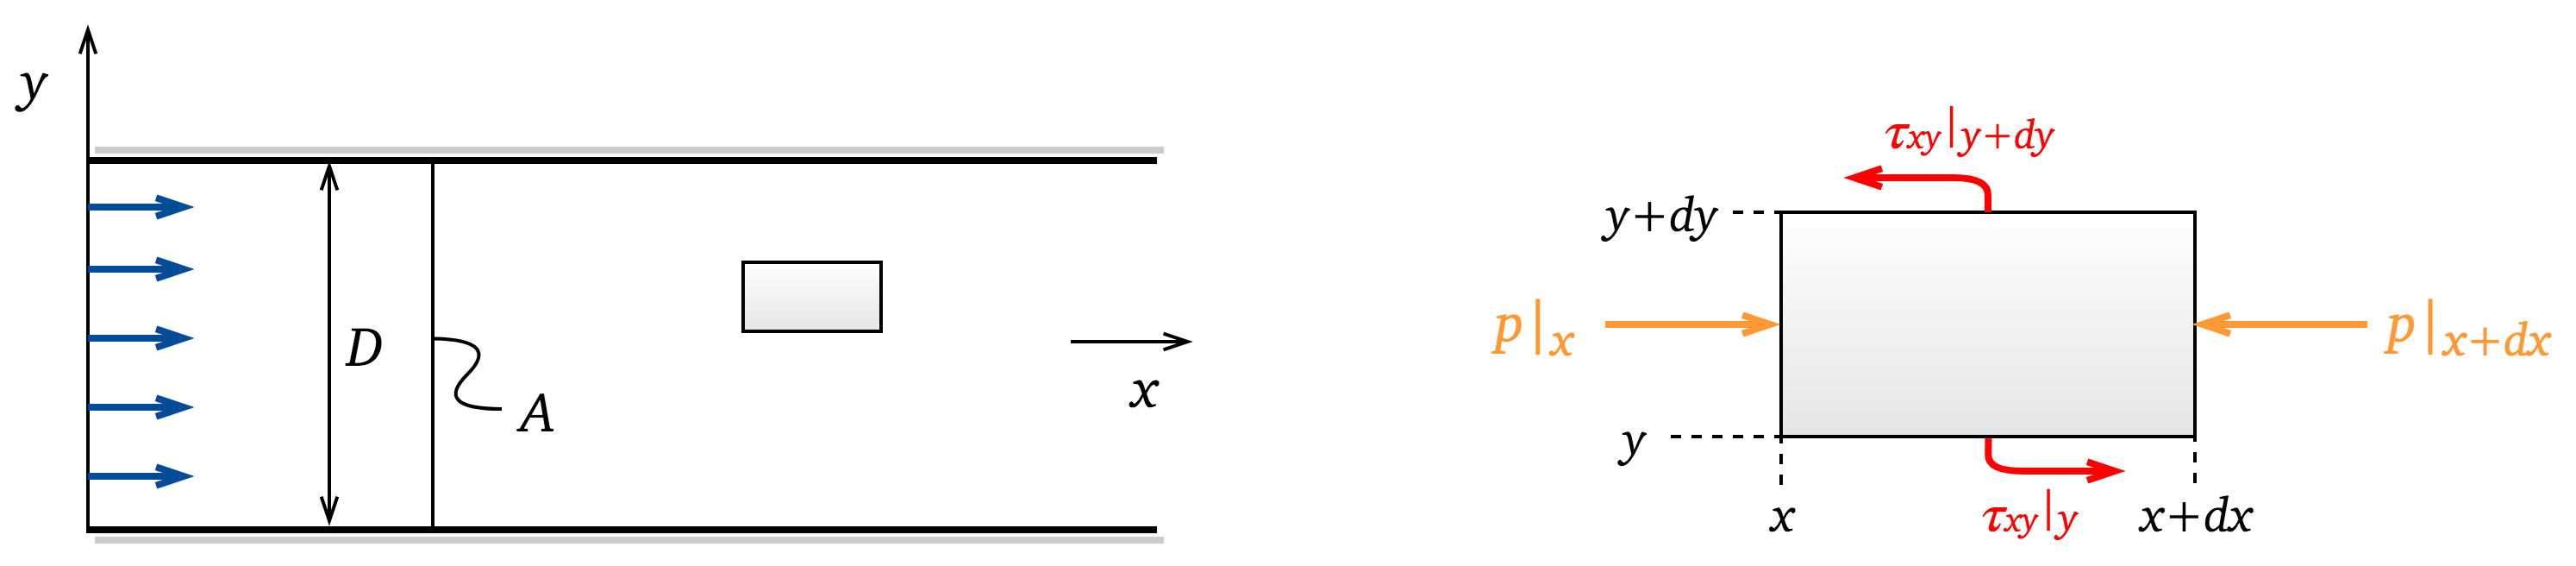
\includegraphics[width=15cm]{poiseuille-fluid-element}
\caption{Flow between two parallel plates with an infinitesimal fluid element.}			
\label{fig:poiseuille-fluid-element}
\end{figure}

We also have three boundary conditions. Due to a no-slip condition we assume that the velocity at the very surface of the plates is zero: $u(-D/2) = 0$ and $u(D/2) = 0$. Due to symmetry of the flow we assume that there cannot be any net momentum transfer between the upper half and the lower half of the channel. Hence, the shear stress exactly in the middle of the channel is zero: $\tau_{xy}(0) = 0$.

Steady state momentum (force) balance, taking into account pressure and shear forces on a single infinitesimal fluid element:

\begin{equation}
0 = p|_x B dy - p|_{x+dx} B dy + \tau_{xy}|_y B dx - \tau_{yx}|_{y+dy} B dx
\end{equation}

Dividing both sides by the width $B$ and by $dx dy$ we obtain:

\begin{equation}
0 = \frac{p|_x  - p|_{x+dx}}{dx}  + \frac{\tau_{xy}|_y  - \tau_{yx}|_{y+dy}}{dy} 
\end{equation}

Now we notice that $\frac{p|_x  - p|_{x+dx}}{dx}$ is in fact equal to $-\frac{dp}{dx}$ (in a limit as $dx \rightarrow 0$), since it is an incremental change in pressure function value per incremental distance $dx$. Similar thing can be said about $\frac{\tau_{xy}|_y  - \tau_{yx}|_{y+dy}}{dy}$ which is equal to $-\frac{d \tau_{xy}}{dy}$. We can thus further simplify:

\begin{equation}
\frac{d \tau_{xy}}{dy} = - \frac{dp}{dx} = \text{const}
\end{equation}

Integrating the above equation and applying the initial condition for the shear stress $\tau_{xy}(0) = 0$:

\begin{equation} \label{eq:shear-poiseuille}
\tau_{xy}(y)= - \frac{dp}{dx} y
\end{equation}

Adding a constitutive relation for Newtonian fluids we can further relate pressure and velocity. From the Newton's law we know also that:

\begin{equation} \label{eq:shear-newton}
\tau_{xy}(y)= - \mu \frac{du}{dy}
\end{equation}

You may look at this in such a way: the equation \ref{eq:shear-poiseuille} is a special case in which the shear stresses have been related to the driving force in the Poiseuille flow - the pressure gradient. The equation \ref{eq:shear-newton} is a general description of any shear stress $\tau_{xy}$, where it is linked to velocity gradients, no matter what the cause for this velocity gradient is! It just so happens that in the case of a Poiseuille flow between two parallel plates this cause is the pressure drop:

\begin{equation}
- \mu \frac{du}{dy} = - \frac{dp}{dx} y
\end{equation}

Integrating one more time the above relation and applying the no-slip boundary conditions we get:

\begin{equation}
u(y) = \frac{1}{2 \mu} \frac{dp}{dx} (y^2 - (D/2)^2)
\end{equation}


% - - - - - - - - - - - - - - - - - - - - - - - - - - - - - - - - - - - - - - - - - - - - - - - - 
\chapter{Drag force}

The mathematical description of the drag force begins with making a guess. It is an intuitive guess which answers the question: what physical quantities affect the value of the drag force on an object moving through a fluid? The thought process done on this question gives the following four quantities:

relative fluid-object velocity $\upsilon$ \,\,\,\,\,\,\,\,\,\,\,\,\,\,\,  fluid density $\rho$ \,\,\,\,\,\,\,\,\,\,\,\,\,\,\, fluid viscosity $\mu$ \,\,\,\,\,\,\,\,\,\,\,\,\,\,\, geometry of an object $D$

We assume that the drag force is a combination of these quantities to some yet unknown powers and we use dimensional analysis to find those powers.

\begin{equation}
F_D = \upsilon^a \rho^b \mu^c D^d
\label{eq:drag_force}
\end{equation}

Writing out the units of the above equation we get:

\begin{equation*}
\Big[ \frac{kg \cdot m}{s^2} \Big] = \Big[ \frac{m}{s} \Big]^a \cdot \Big[ \frac{kg}{m^3} \Big]^b \cdot \Big[ \frac{kg}{m \cdot s} \Big]^c \cdot \Big[ m \Big]^d
\end{equation*}

Shuffling around a bit:

\begin{equation*}
kg \cdot m \cdot s^{-2} = kg^{b+c} \cdot m^{a -3b - c + d} \cdot s^{-a - c}
\end{equation*}

Hence:

$1 = b+c$

$1 = a - 3b - c + d$

$-2 = - a - c$

The simple fact that this set of equations cannot be solved exactly (there is four  uknown powers and only three equations) is going to call experiment for help, which you will notice in the next few passages.

Let's then write the set of equations by means of one of the unknowns $c$:

$a = 2 - c$

$b = 1 - c$

$d = 2 - c$

\newpage

Subsituting back to the equation \ref{eq:drag_force} we get:

\begin{equation}
F_D = \upsilon^{2 - c} \rho^{1 - c} \mu^c D^{2 - c} 
\label{eq:drag_force_powers}
\end{equation}

Structuring the equation still a bit gives:

\begin{equation}
F_D = \upsilon^2 \rho D^2 \cdot \Big[ \frac{\upsilon \rho D}{\mu} \Big]^{-c}
\label{eq:drag_force_powers}
\end{equation}

It always feels comfortable to find the Reynolds number in your equation, so there it is:

\begin{equation}
F_D = \upsilon^2 \rho D^2 Re^{-c}
\label{eq:drag_force_powers}
\end{equation}

We get finally that the drag force is proportional to some unknown power of the Reynolds number.


In fact, we will not leave it there yet, since there is an interesting last point to say. Instead of the above equation, we will say that the drag force is proportional to some unknown function $C_D$ of the Reynolds number. We also recognise that we may rewrite the quantity $\upsilon^2 \rho$ as the dynamic pressure $\frac{\upsilon^2 \rho}{2}$, since multiplying the right hand side by $\frac{1}{2}$ will not spoil the dimensional equality of both sides. The quantity $D^2$ has got the unit of area, so we exchange it for the quantity $A_{\perp}$, representing the frontal area of an object. The equation for the drag force becomes:

\begin{equation}
F_D = \frac{\upsilon^2 \rho}{2} A_{\perp} C_D (Re)
\label{eq:drag_force_powers}
\end{equation}

The unknown function $C_D (Re)$ is called the \textbf{drag coefficient}. That is where we call for experiment.

Questions:

What would have happened if we wrote the powers in terms of some power other than $c$?










% - - - - - - - - - - - - - - - - - - - - - - - - - - - - - - - - - - - - - - - - - - - - - - - - 
\chapter{Circulation}



Circulation is defined as:

\begin{equation}
\Gamma = \oint_C \vec{\upsilon} \cdot \vec{dl}
\end{equation}

The dot product, $\vec{\upsilon} \cdot \vec{dl}$, returns a scalar which is expressing ''how much`` in the direction of the other vector is this vector.

\begin{figure}[H]
\centering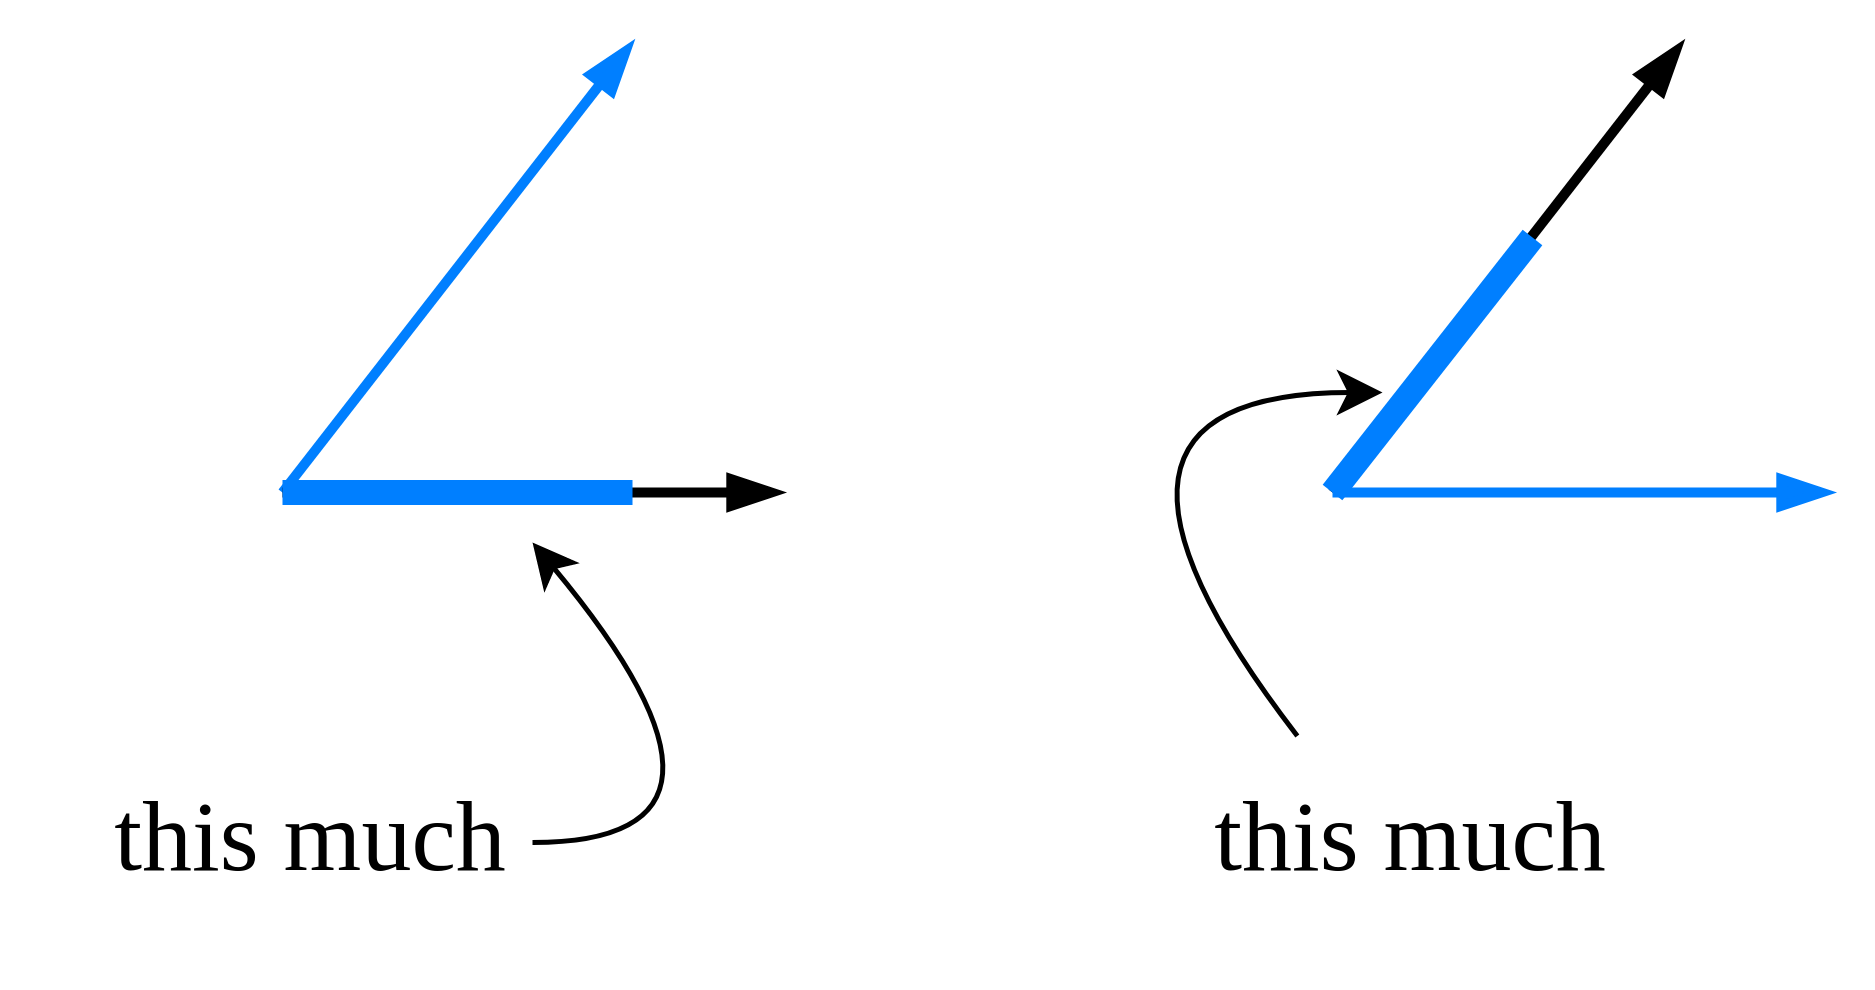
\includegraphics[width=5cm]{circulation_dot_prod}
\caption{Dot product of two vectors.}			
\label{fig:circulation-dot-product}
\end{figure}

When they are $\perp$, the dot product is zero.

In the concept of circulation, we ask ''how much`` at any point on the curve $C$ the velocity vector at that point is in the direction of the curve's geometry. Now, that doesn't yet sound as something to do with ''circulating``. For the moment, I would think that it's more of an ''on-trackness``. Something, that in real world would be for instance the measure of how much the vehicle's velocity is in the direction of the road geometry (which we would hope is all of it!).

But to start 
, notice an important detail of ''$\circ$`` on the integral symbol, which signals that the curve should be a closed curve -- a loop -- although not necessarily a perfect circle.

When you perform integration, which means summing up every little $\vec{\upsilon} \cdot \vec{dl}$ as you go around the loop, you count ''how much`` at every point on the loop, the velocity vector at these points is in the direction of the loop's geometry (at these points).

If we were to place a small particle at some starting point $P$ on the loop, the circulation would tell us ''how much`` the velocity field which this particle is subjected to, is tending to move that particle around the loop.

It can be very intuitive when you take a look at these two pictures:





It's no surprise that when the velocity is everywhere perpendicular to the loop's geometry, the circulation around the loop is zero. If you were to place a particle at any point on the loop, such velocity field would act to immediately displace the particle off the loop. Therefore, the particle would have no way of ''circulating`` around the loop.

On the other extreme is the case when the velocity field is everywhere tangent to the loop's geometry. Anywhere the particle goes on the loop, the velocity at that point would act to keep the particle moving around the loop.

Questions:

\begin{enumerate}
\item Why closed loop? Would it have any meaning if we calculated circulation along any general spline?

\item How to chose loops so that the circulation we calculate is of the most meaning to us?

\item What does the zero, positive, negative circulation mean?

\item Can circulation be infinite?

\item For what velocity field, $\vec{\upsilon}$, and the corresponding loop, $C$, is circulation zero?
\end{enumerate}



% - - - - - - - - - - - - - - - - - - - - - - - - - - - - - - - - - - - - - - - - - - - - - - - - 
%\chapter{Vorticity}

%
\begin{enumerate}
\item Why is vorticity concept needed? Isn't it something kind of like circulation?

\end{enumerate}


% - - - - - - - - - - - - - - - - - - - - - - - - - - - - - - - - - - - - - - - - - - - - - - - - 
%\chapter{Stoke's theorem}

%




% - - - - - - - - - - - - - - - - - - - - - - - - - - - - - - - - - - - - - - - - - - - - - - - - 
%\chapter{Nondimensionalizing}

%
What's with the nondimensionalizing? 

% - - - - - - - - - - - - - - - - - - - - - - - - - - - - - - - - - - - - - - - - - - - - - - - - 
%\chapter{Conservation of mass}

%While the Navier-Stokes equations\footnote{See Chapter~\ref{chap:N-S}.} are all the rage in fluid dynamics, with people tattooing them on their bodies, I'm a big fan of the continuity equation for its modesty! The right-hand-side of the Navier-Stokes equations can become arbitrarily messy if we need to account for all the different sources of momentum change. But nothing can be taken away or added to the continuity equation. It's perfect just the way it is, and yet it describes one of the fundamental conservation laws that mass cannot be lost nor created. Powerful stuff, huh? That's its modest beauty that I hope to show you in this chapter!


In this chapter we present the derivation of the conservation of mass equation, otherwise known as the \textbf{continuity equation}. We begin by writing out the overall mass balance inside any control volume CV. The net change of mass inside the control volume is equal to the mass flowing into the CV minus the mass flowing out of the CV. Note here, that when the net change of mass in a CV is not zero (unsteady case), it can only be due to either compression (more mass flowing in than flowing out) or decompression (more mass flowing out than flowing in). The general mass balance is:

\begin{equation} \label{eq:net_change}
\text{net change} = \text{flow in} - \text{flow out}
\end{equation}

\section{Mass flow rate}

\section{Derivation using control volume}

We are going to write out the RHS of the equation \ref{eq:net_change} as the difference between mass flow rate in and mass flow rate out in three Cartesian directions.

In the $x$-direction:

\begin{equation}
\Big( \rho u - \frac{\partial (\rho u)}{\partial x} \frac{dx}{2} \Big) dy dz - \Big( \rho u + \frac{\partial (\rho u)}{\partial x} \frac{dx}{2} \Big) dy dz = - \frac{\partial (\rho u)}{\partial x} dx dy dz
\end{equation}

In the $y$-direction:

\begin{equation}
\Big( \rho v - \frac{\partial (\rho v)}{\partial y} \frac{dy}{2} \Big) dx dz - \Big( \rho v + \frac{\partial (\rho v)}{\partial y} \frac{dy}{2} \Big) dx dz = - \frac{\partial (\rho v)}{\partial y} dy dx dz
\end{equation}

In the $z$-direction:

\begin{equation}
\Big( \rho w - \frac{\partial (\rho w)}{\partial z} \frac{dz}{2} \Big) dx dy - \Big( \rho w + \frac{\partial (\rho w)}{\partial z} \frac{dz}{2} \Big) dx dy = - \frac{\partial (\rho w)}{\partial z} dz dx dy
\end{equation}

The net change in time of mass can be written as:

\begin{equation}
\frac{\partial \rho}{dt} dx dy dz
\end{equation}

Putting all the terms together into equation \ref{eq:net_change} we obtain:

\begin{equation}
\frac{\partial \rho}{dt} dx dy dz = - \frac{\partial (\rho u)}{\partial x} dx dy dz - \frac{\partial (\rho v)}{\partial y} dy dx dz - \frac{\partial (\rho w)}{\partial z} dz dx dy
\end{equation}

Dividing both sides by $dx dy dz$ we get:

\begin{equation} \label{eq:continuity_general}
\frac{\partial \rho}{dt} = - \frac{\partial (\rho u)}{\partial x} - \frac{\partial (\rho v)}{\partial y} - \frac{\partial (\rho w)}{\partial z}
\end{equation}

Lastly, we can observe that the divergence of the quantity $\rho \vec{V}$ is:

\begin{equation}
\nabla (\rho \vec{V}) = \nabla (\rho \langle u, v, w \rangle) = \nabla \langle \rho u, \rho v, \rho w \rangle = \frac{\partial (\rho u)}{\partial x} + \frac{\partial (\rho v)}{\partial y} + \frac{\partial (\rho w)}{\partial z}
\end{equation}

So in the end, we can further write the RHS of the equation \ref{eq:continuity_general} in a shorter format as:

\begin{equation} \label{eq:continuity_divergence}
\frac{\partial \rho}{dt} = - \nabla \cdot (\rho \vec{V})
\end{equation}

\section{Special cases of density function}

So let's push the continuity equations to its limits! Let's see how many different physical scenarios can it describe.
In the most general case, the density is a function of time and space, $\rho = \rho(t, x, y, z)$, and the Eq.~(\ref{eq:continuity_divergence}) is written out for the most general case. This describes the compressible, unsteady flow. But special cases can be defined when certain restrictions are imposed on the density function.

\textbf{Compressible, steady flow}

First, when the density is only a function of position, $\rho = \rho(x,y,z)$, and does not change in time at any point in the flow field, we arrive at the steady-state condition where the derivative $\frac{\partial \rho}{dt} = 0$.

The continuity equation then becomes:

\begin{equation} \label{eq:continuity_stst}
0 = - \nabla \cdot (\rho  \vec{V})
\end{equation}

\textbf{Incompressible, unsteady flow}

When we assume that the density is constant in space, it can be taken out front of the divergence operator and the incompressible continuity equation is:

\begin{equation} \label{eq:continuity_incompressible}
\frac{\partial \rho}{dt} = - \rho \nabla \cdot \vec{V}
\end{equation}

The above equation corresponds to the density that is constant throughout the flow field at any moment in time, but can change in time in the entire flow field.

\textbf{Incompressible, steady flow}

The steady flow can be further combined with the incompressible condition, which disables the density to change both in time and space. The stead-state incompressible continuity equation then becomes:

\begin{equation} \label{eq:continuity_stst_incompressible}
0 = \nabla \cdot \vec{V}
\end{equation}

or writing the above equation with the use of partial differentiation operator:

\begin{equation}
\frac{\partial u}{\partial x} + \frac{\partial v}{\partial y} + \frac{\partial w}{\partial z} = 0
\end{equation}




\section{Divergence theorem and a different way of looking at the conservation of mass}

% - - - - - - - - - - - - - - - - - - - - - - - - - - - - - - - - - - - - - - - - - - - - - - - - 
%\chapter{Gauss's law}

%Differentiation is a way to make discrete things continuous.

% - - - - - - - - - - - - - - - - - - - - - - - - - - - - - - - - - - - - - - - - - - - - - - - - 
%\chapter{Reynolds number}

%I this chapter we travel a journey through the many faces of the Reynolds number.

% - - - - - - - - - - - - - - - - - - - - - - - - - - - - - - - - - - - - - - - - - - - - - - - - 
\chapter{Constitutive equations}

In case you need to understand the constitutive equations for use in the Navier-Stokes equations, you may skip this chapter for now and come back to it once you are in the \textit{Constitutive equations} section inside the Navier-Stokes equations chapter.

% - - - - - - - - - - - - - - - - - - - - - - - - - - - - - - - - - - - - - - - - - - - - - - - - 
\chapter{The Navier-Stokes equations}

The Navier-Stokes equations represent the momentum balance on an infinitesimal fluid volume. They state that the sum of forces acting on a fluid volume is equal to the change in momentum for that volume (Newton's second law).

\section{Incompressible Navier-Stokes}

In a three-dimensional, incompressible, unsteady flow we have:

$x$-direction:

\begin{equation} \label{eq:NS_x}
\rho g_x - \frac{\partial P}{\partial x} + \mu \Big( \frac{\partial^2 u}{\partial x^2} + \frac{\partial^2 u}{\partial y^2} + \frac{\partial^2 u}{\partial z^2}\Big) = \rho \Big( \frac{\partial u}{\partial t} + u \frac{\partial u}{\partial x} + v \frac{\partial u}{\partial y} + w \frac{\partial u}{\partial z} \Big)
\end{equation}

$y$-direction:

\begin{equation} \label{eq:NS_y}
\rho g_y - \frac{\partial P}{\partial y} + \mu \Big( \frac{\partial^2 v}{\partial x^2} + \frac{\partial^2 v}{\partial y^2} + \frac{\partial^2 v}{\partial z^2}\Big) = \rho \Big( \frac{\partial v}{\partial t} + u \frac{\partial v}{\partial x} + v \frac{\partial v}{\partial y} + w \frac{\partial v}{\partial z} \Big)
\end{equation}

$z$-direction:

\begin{equation} \label{eq:NS_z}
\rho g_z - \frac{\partial P}{\partial z} + \mu \Big( \frac{\partial^2 w}{\partial x^2} + \frac{\partial^2 w}{\partial y^2} + \frac{\partial^2 w}{\partial z^2}\Big) = \rho \Big( \frac{\partial w}{\partial t} + u \frac{\partial w}{\partial x} + v \frac{\partial w}{\partial y} + w \frac{\partial w}{\partial z} \Big)
\end{equation}

\section{Derivation}

Sum of the forces is written on the LHS of the above equations. The total change in momentum is written on the RHS of the above equations.

\subsection{RHS}

In the most general case, the velocity vector $\vec{V} = \langle u, v, w \rangle$ is a function of time and position. We write therefore: $\vec{V}(t, x, y, z) = \langle u(t, x, y, z), v(t, x, y, z), w(t, x, y, z) \rangle $.

The acceleration component is described as the time derivative of the corresponding velocity component. If you were to take the derivative with respect to time of any of the above components of the velocity vector, it would become due to chain rule:

\begin{equation}
a_x = \frac{\partial u(t,x,y,z)}{\partial t} = \frac{\partial u}{\partial t} \frac{\partial t}{\partial t} + \frac{\partial u}{\partial x} \frac{\partial x}{\partial t} + \frac{\partial u}{\partial y} \frac{\partial y}{\partial t} + \frac{\partial u}{\partial z} \frac{\partial z}{\partial t}
\end{equation}

Observe then, that $\frac{\partial t}{\partial t} = 1$, $\frac{\partial x}{\partial t} = u$, $\frac{\partial y}{\partial t} = v$, $\frac{\partial z}{\partial t} = w$.

We have therefore for all three components:

\begin{equation}
a_x = \frac{\partial u(t,x,y,z)}{\partial t} = \frac{\partial u}{\partial t} + u \frac{\partial u}{\partial x} + v \frac{\partial u}{\partial y} + w \frac{\partial u}{\partial z}
\end{equation}

\begin{equation}
a_y = \frac{\partial v(t,x,y,z)}{\partial t} = \frac{\partial v}{\partial t} + u \frac{\partial v}{\partial x} + v \frac{\partial v}{\partial y} + w \frac{\partial v}{\partial z}
\end{equation}

\begin{equation}
a_z = \frac{\partial w(t,x,y,z)}{\partial t} = \frac{\partial w}{\partial t} + u \frac{\partial w}{\partial x} + v \frac{\partial w}{\partial y} + w \frac{\partial w}{\partial z}
\end{equation}

The terms $\frac{\partial u}{\partial t}$, $\frac{\partial v}{\partial t}$, $\frac{\partial w}{\partial t}$ are called \textbf{local accelerations}, and the remaining terms where the derivatives are taken with respect to spacial coordinates are called \textbf{convective accelerations}\footnote{See the chapter on Material Derivative for more understanding of the local and convective terms.}. The names \textit{local} and \textit{convective} carry a lot of meaning here, although initially it might be hard to see. 

The word \textit{convective} means that it is a quantity that depends on traveling to other regions - in other words - it depends on position. It is going to change due to the fact that the fluid element has traveled to a new place.

The word \textit{local}, on the other hand, suggests that it is a quantity that is intrinsic to the particular fluid element and its change is independent of the particle's position in space. The \textit{local} quantity can change in a fluid element, but solely "in itself" as the time pass (or \textit{locally} and that will happen independent of where the fluid particle travels to). 

Notice that this logic fits into how these derivatives look like. The convective terms are all derivatives with respect to position - they account for a change in velocity components due to change in coordinates. The local terms are all derivatives with respect to time - they just change by itself as the time change and position is irrelevant.

The above equations represent the acceleration components. These components are present in the RHS of the Navier-Stokes equations [\ref{eq:NS_x} - \ref{eq:NS_z}].

The standard way to write the Newton's second law is that the sum of the forces equals mass multiplied by acceleration. Since the Navier-Stokes equations are written per volume basis, the change in momentum (or the mass multiplied by acceleration) is written per unit of volume, so:

\begin{equation}
\frac{dm}{dV} a_x = \frac{dm}{dV} \frac{\partial u(t,x,y,z)}{\partial t} = \rho \frac{\partial u(t,x,y,z)}{\partial t}
\end{equation}

Multiplying all the acceleration components by the density $\rho$ we are going to obtain the full description for the change in momentum per unit of volume:

\begin{equation}
\rho a_x = \rho \frac{\partial u(t,x,y,z)}{\partial t} = \rho \frac{\partial u}{\partial t} + \rho  u \frac{\partial u}{\partial x} + \rho v \frac{\partial u}{\partial y} + \rho w \frac{\partial u}{\partial z}
\end{equation}

\begin{equation}
\rho a_y = \rho \frac{\partial v(t,x,y,z)}{\partial t} = \rho \frac{\partial v}{\partial t} + \rho u \frac{\partial v}{\partial x} + \rho v \frac{\partial v}{\partial y} + \rho w \frac{\partial v}{\partial z}
\end{equation}

\begin{equation}
\rho a_z = \rho \frac{\partial w(t,x,y,z)}{\partial t} = \rho \frac{\partial w}{\partial t} + \rho u \frac{\partial w}{\partial x} + \rho v \frac{\partial w}{\partial y} + \rho w \frac{\partial w}{\partial z}
\end{equation}

This concludes the derivation and explanation of the RHS of the Navier-Stokes equations stated at the beginning of this chapter.


\subsection{LHS}

We are now going to crunch the LHS of the Navier-Stokes equations - the sum of the forces acting on a unit volume of fluid. There are two types of forces taken into account here: \textbf{body forces} (gravity) and \textbf{surface forces} (forces due to pressure difference and dissipative forces due to viscosity).

\subsubsection{Gravity forces}

The body forces due to gravity are perhaps the most intuitive to figure out. In order to construct the gravity force $F_{g, x}$ on a fluid element, we multiply mass of that element by gravitational acceleration. Inside the Navier-Stokes equations it is not any different. We have the terms: $\rho g_x$, $\rho g_y$, $\rho g_z$, that represent exactly that idea, except they are again written on a per volume basis.

\begin{equation}
\frac{d F_{g, x}}{dV} = \frac{dm}{dV} g_x =  \rho g_x
\end{equation}

\begin{equation}
\frac{d F_{g, y}}{dV} = \frac{dm}{dV} g_y =  \rho g_y
\end{equation}

\begin{equation}
\frac{d F_{g, z}}{dV} = \frac{dm}{dV} g_z =  \rho g_z
\end{equation}

\subsubsection{Surface forces}

The surface stresses can be represented by the \textbf{stress tensor}:

\begin{equation}
\bm{\sigma}_{IN} = \left(
\begin{matrix} 
\sigma_{xx} & \sigma_{xy} & \sigma_{xz} \\
\sigma_{yx} & \sigma_{yy} & \sigma_{yz} \\
\sigma_{zx} & \sigma_{zy} & \sigma_{zz}
\end{matrix}
\right)
\,\,\,\,\,\,\,\,\,\,\,\,
\bm{\sigma}_{OUT} = \left(
\begin{matrix} 
\sigma_{xx} + \frac{\partial \sigma_{xx}}{\partial x}dx & \sigma_{xy} + \frac{\partial \sigma_{xy}}{\partial x}dx & \sigma_{xz} + \frac{\partial \sigma_{xz}}{\partial x}dx \\
\sigma_{yx} + \frac{\partial \sigma_{yx}}{\partial y}dy & \sigma_{yy} + \frac{\partial \sigma_{yy}}{\partial y}dy & \sigma_{yz} + \frac{\partial \sigma_{yz}}{\partial y}dy \\
\sigma_{zx} + \frac{\partial \sigma_{zx}}{\partial z}dz & \sigma_{zy} + \frac{\partial \sigma_{zy}}{\partial z}dz & \sigma_{zz} + \frac{\partial \sigma_{zz}}{\partial z}dz 
\end{matrix}
\right)
\end{equation}

The net force on the fluid element resulting from the surface stresses comes from the difference between stresses on two opposing sides of the fluid element. Therefore we are going to look at the value of:

\begin{equation}
\bm{\sigma}_{OUT} - \bm{\sigma}_{IN} = \left(
\begin{matrix} 
 \frac{\partial \sigma_{xx}}{\partial x}dx & \frac{\partial \sigma_{xy}}{\partial x}dx & \frac{\partial \sigma_{xz}}{\partial x}dx \\
\frac{\partial \sigma_{yx}}{\partial y}dy & \frac{\partial \sigma_{yy}}{\partial y}dy & \frac{\partial \sigma_{yz}}{\partial y}dy \\
\frac{\partial \sigma_{zx}}{\partial z}dz & \frac{\partial \sigma_{zy}}{\partial z}dz & \frac{\partial \sigma_{zz}}{\partial z}dz 
\end{matrix}
\right)
\end{equation}

Since we are interested in forces resulting from these stresses, we need to multiply the above values by the areas of the corresponding surfaces on which these stresses act.

\begin{equation}
F_{\sigma} = \left(
\begin{matrix} 
\frac{\partial \sigma_{xx}}{\partial x}dx dy dz & \frac{\partial \sigma_{xy}}{\partial x}dx dx dz & \frac{\partial \sigma_{xz}}{\partial x}dx dx dy \\
\frac{\partial \sigma_{yx}}{\partial y}dy dy dz & \frac{\partial \sigma_{yy}}{\partial y}dy dx dz & \frac{\partial \sigma_{yz}}{\partial y}dz dx dy\\
\frac{\partial \sigma_{zx}}{\partial z}dx dy dz & \frac{\partial \sigma_{zy}}{\partial z}dy dx dz & \frac{\partial \sigma_{zz}}{\partial z}dz dx dy
\end{matrix}
\right)
\end{equation}

And lastly, we will write the forces per unit of volume:

\begin{equation} \label{eq:forces_sigma}
f_{\sigma} = \left(
\begin{matrix} 
\frac{\partial \sigma_{xx}}{\partial x} & \frac{\partial \sigma_{xy}}{\partial x} & \frac{\partial \sigma_{xz}}{\partial x} \\
\frac{\partial \sigma_{yx}}{\partial y} & \frac{\partial \sigma_{yy}}{\partial y} & \frac{\partial \sigma_{yz}}{\partial y} \\
\frac{\partial \sigma_{zx}}{\partial z} & \frac{\partial \sigma_{zy}}{\partial z} & \frac{\partial \sigma_{zz}}{\partial z}
\end{matrix}
\right)
\end{equation}

Since the pressure $P$ is often a variable of interest when it comes to fluids, it is worth decomposing the stress tensor to two terms:

\begin{equation}
\bm{\sigma}_{ij} = \left(
\begin{matrix} 
-P & 0 & 0  \\
0 & -P & 0 \\
0 & 0 & -P 
\end{matrix}
\right) + 
\left(
\begin{matrix} 
\tau_{xx} & \tau_{xy} & \tau_{xz} \\
\tau_{yx} & \tau_{yy} & \tau_{yz} \\
\tau_{zx} & \tau_{zy} & \tau_{zz}
\end{matrix}
\right)
\end{equation}

The above pressure $P$ is such that for a fluid at rest the stress tensor is simply:

\begin{equation}
\bm{\sigma}_{ij} = \left(
\begin{matrix} 
-P & 0 & 0  \\
0 & -P & 0 \\
0 & 0 & -P 
\end{matrix}
\right)
\end{equation}

The matrix with $\tau$-terms is called \textbf{viscous stress tensor}. In a special case when fluid is inviscid this tensor is zero.

\begin{equation}
\bm{\tau}_{ij} = 
\left(
\begin{matrix} 
\tau_{xx} & \tau_{xy} & \tau_{xz} \\
\tau_{yx} & \tau_{yy} & \tau_{yz} \\
\tau_{zx} & \tau_{zy} & \tau_{zz}
\end{matrix}
\right)
\end{equation}

We can now write the forces per unit volume (eq. \ref{eq:forces_sigma}) as:

\begin{equation} \label{eq:forces_sigma_2}
f_{\sigma} = \left(
\begin{matrix} 
\frac{\partial (\tau_{xx} - P)}{\partial x} & \frac{\partial \tau_{xy}}{\partial x} & \frac{\partial \tau_{xz}}{\partial x} \\
\frac{\partial \tau_{yx}}{\partial y} & \frac{\partial (\tau_{yy} - P)}{\partial y} & \frac{\partial \tau_{yz}}{\partial y} \\
\frac{\partial \tau_{zx}}{\partial z} & \frac{\partial \tau_{zy}}{\partial z} & \frac{\partial (\tau_{zz} - P)}{\partial z}
\end{matrix}
\right)
\end{equation}

The above formulation is convenient because there *might*\footnote{I say *might* because we often deal with Newtonian fluids for which this formulation is known. In short, for Newtonian fluids there is a way to express shear stresses as being proportional to velocity gradients (with viscosity being the proportionality constant). It is analogous to the relation given by Newton:

\begin{equation}
\tau \propto \frac{\partial u}{dy}
\end{equation}

However, when dealing with fluids of a more complex nature than Newtonian fluids, this formulation needs to be found accordingly and the remaining derivation of the equations of motion needs to be updated. The Navier-Stokes equations are presented in this chapter for Newtonian fluids.} exist a known relationship between shear stresses $\tau_{ij}$ and velocity gradients (see chapter on \textit{Constitutive equations} for a more intuitive explanation). Adding such relation allows to finally represent the forces coming from stresses by means of desired parameters: pressure, velocity components and viscosity.




\section{A note about Cauchy's equations}

The Navier-Stokes equation can be thought of as a special case of the Cauchy's equation that is strictly to be used for a specific type of fluid: a Newtonian, incompressible fluid. Cauchy's equation states the law of conservation of linear momentum for any type of fluid. 


\section{Assumptions and limitations}



\newpage


\begin{tikzpicture}
  \node[minimum height=0.8cm,minimum width=16.5cm, fill=lightgray,fill opacity=0.5,rounded
      corners=1ex,font=\fontsize{14pt}{14pt}] (a) {\textit{\textbf{Questions}}};
\end{tikzpicture}

\begin{enumerate}

\item What would the Navier-Stokes equations reduce to for different flow cases?

\end{enumerate}


% - - - - - - - - - - - - - - - - - - - - - - - - - - - - - - - - - - - - - - - - - - - - - - - - 




\chapter*{Appendix}

\newpage
\thispagestyle{empty}

\chapter*{Ending remarks}



\begin{flushright}

%\ \\[6cm]

\includegraphics[width = 100mm]{cover.png}

\setlength{\parskip}{0.1em}
\setlength{\parindent}{0cm}
\ \\[0.5cm]
\textit{The cover photo:}  

View from the coast of Cres island, Croatia, October 2016.
\ \\[0.1cm]
Photo by: J. Aleksanderek $\copyright$
\end{flushright}



\bibliographystyle{apalike}
\bibliography{bibliography}


\end{document}